\documentclass[10pt,letterpaper]{article}
\usepackage[latin1]{inputenc}
\usepackage{amsmath}
\usepackage{amsfonts}
\usepackage{amssymb}

\usepackage{graphicx}
\usepackage{caption}
\usepackage{subcaption}
\usepackage{wrapfig}

\usepackage[left=1.50in, right=1.50in, top=1.50in, bottom=1.50in]{geometry}

\author{Emma Fletcher, Bhargavi Puppola, and Steven Landis\\ with Benjamin Yarmis}
\title{Distributed Robotic Mapping System}
\date{Spring 2012 -- Spring 2013}

\begin{document}
	\maketitle
	
	\hrulefill
	\vfill
	\begin{figure}[h!]
	\centering
		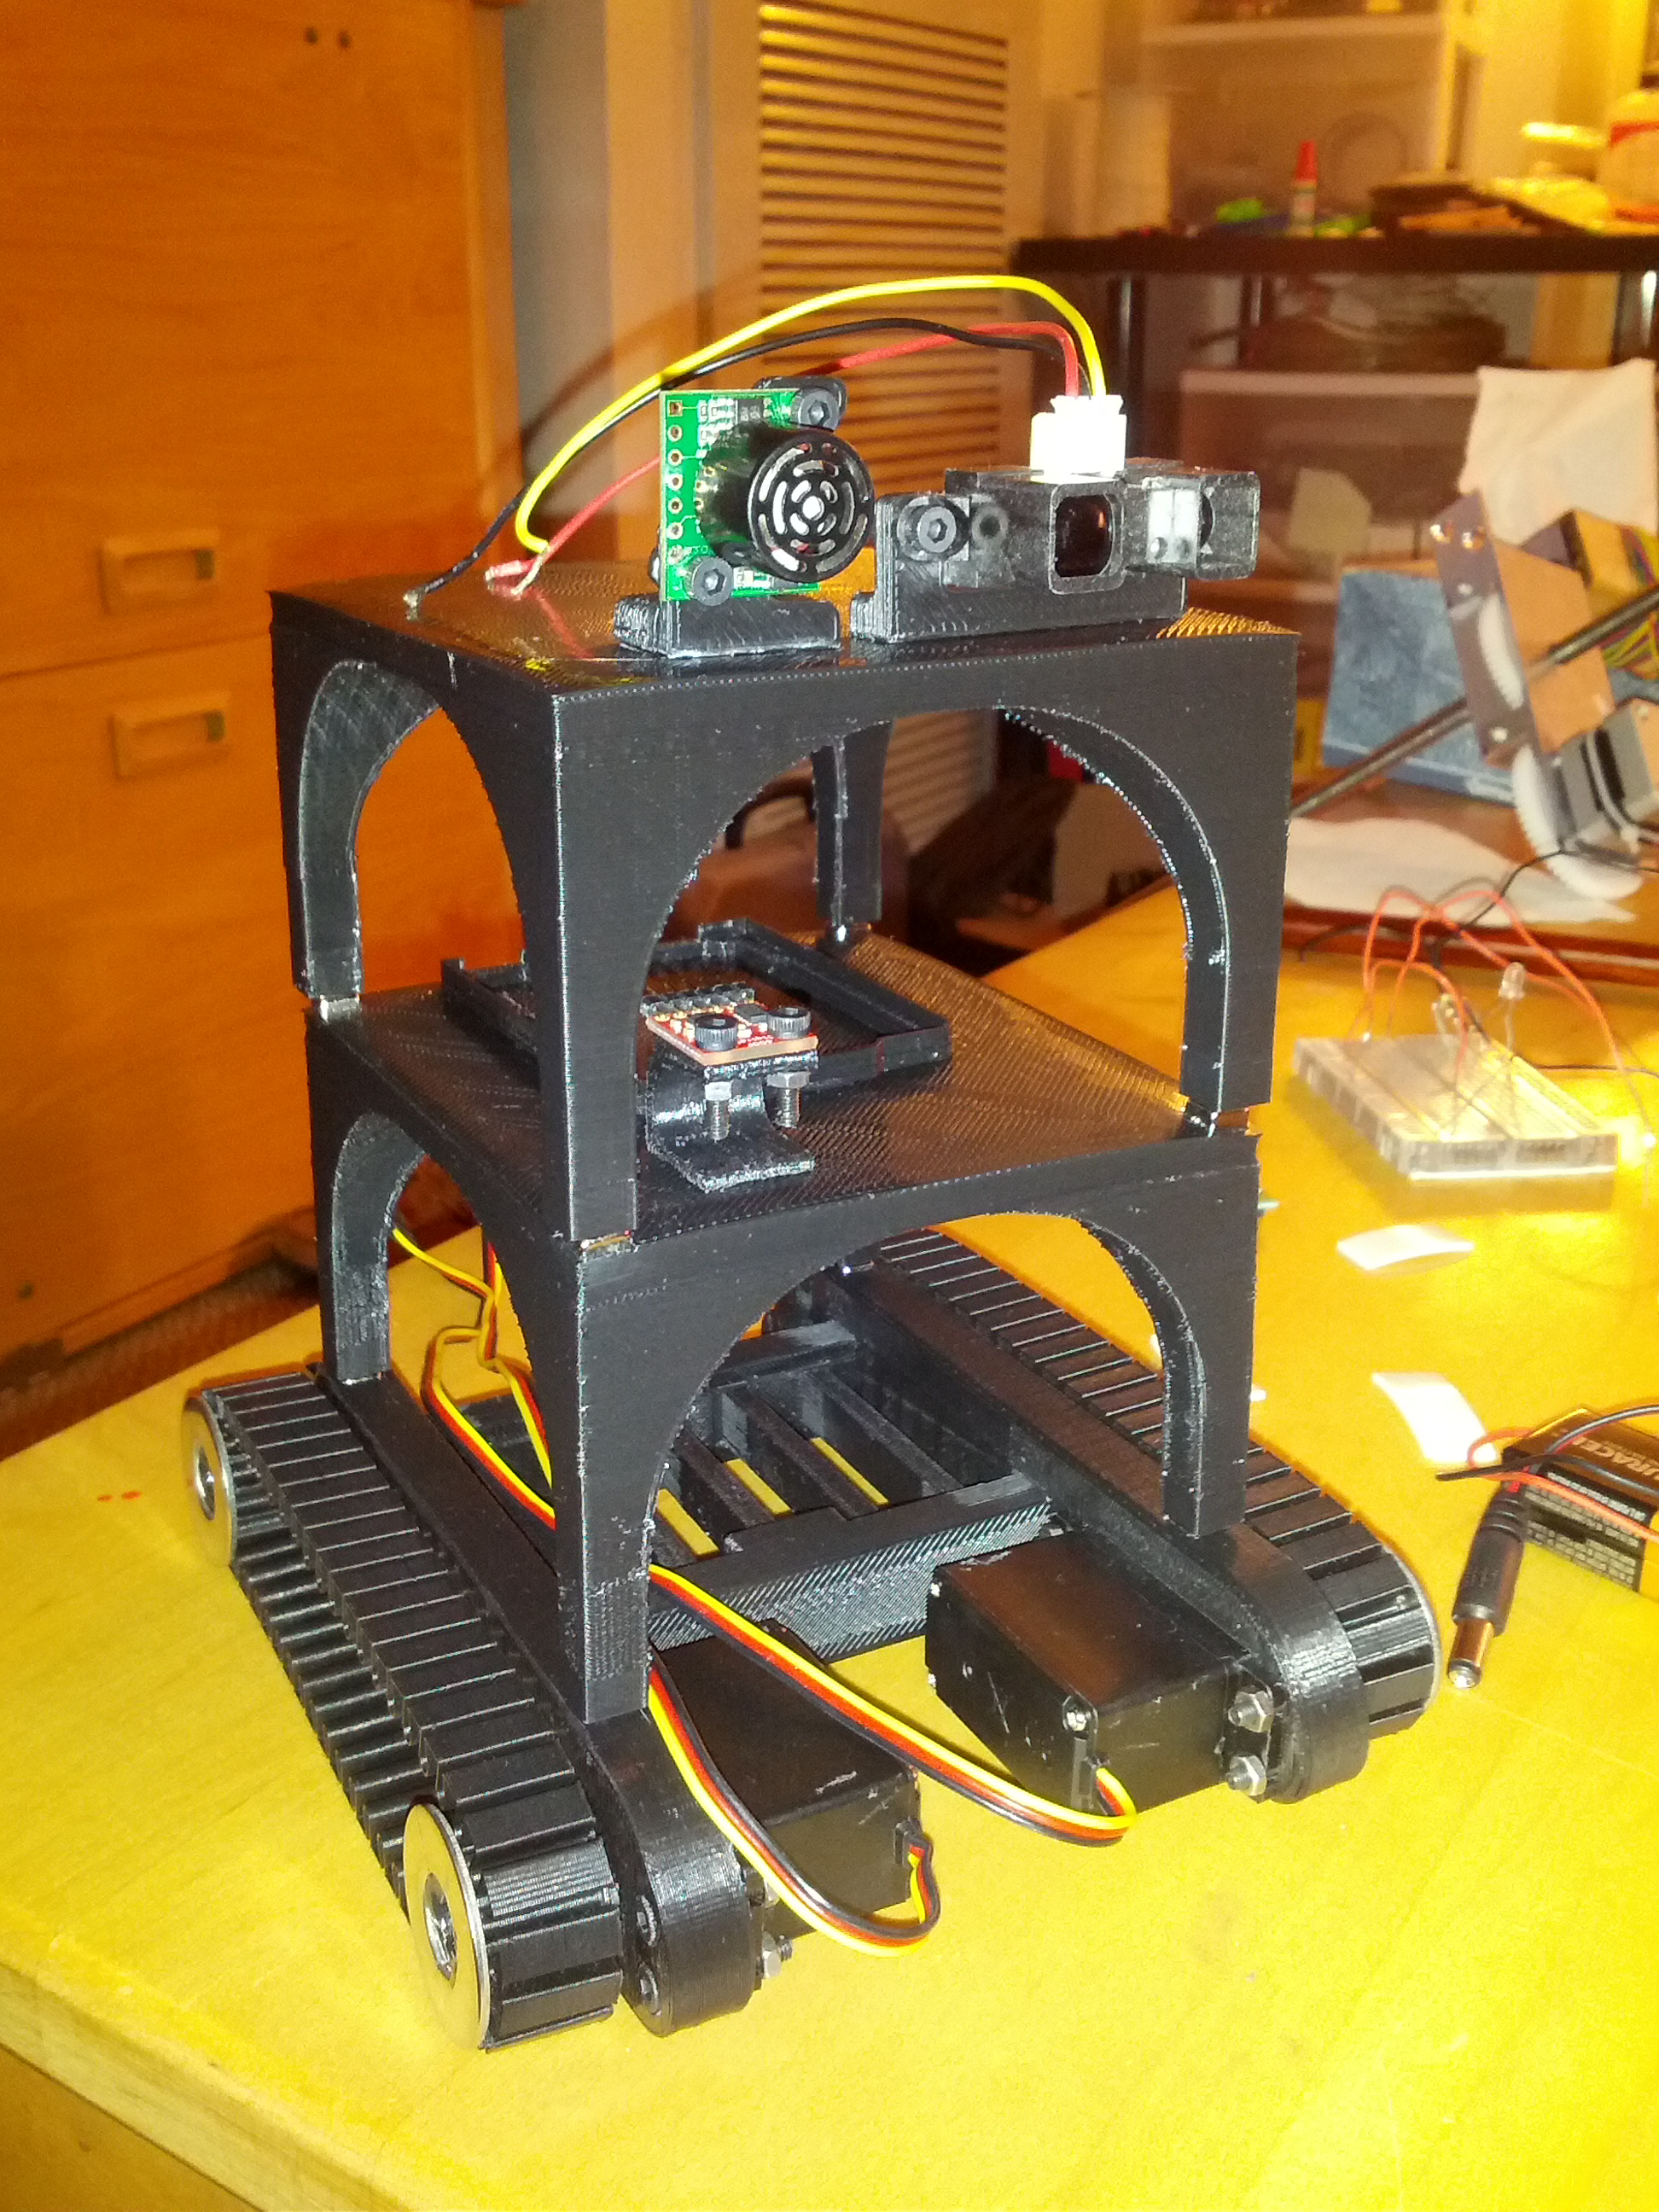
\includegraphics[width=.75\textwidth]{ApolloBuild}
	\end{figure}
	\vfill
	\newpage
	
	\section{Background}
	The ability to autonomously collect data about an unknown environment is critical. When natural disasters occur accurate information about the area is vital for search and rescue teams.  Scientific exploration into dangerous, previously unexplored environments both on earth and in space is valuable to the scientific community. There is a need for a low-cost, accurate, autonomous data collection system for these situations and many others.
	
	\section{Objectives}
	The solution for the exploration of dangerous environments is sending low-cost, versatile, autonomous robots. The Distributed Robotic Mapping System is a versatile group of robots which collect information and relay it to a central server which then creates a three dimensional map for people to study.
	
	\section{Method}
	\begin{wrapfigure}{r}{0.5\textwidth}
		\centering
		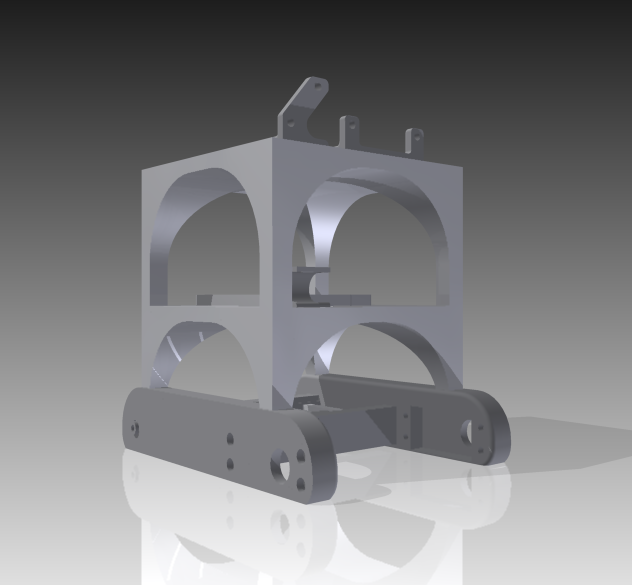
\includegraphics[width=.47\textwidth]{ApolloRender}
		\caption*{Rendering of Design}
	\end{wrapfigure}
		
	The Distributed Robotic Mapping System focuses on three key problems in data collection: cost, scalability and versatility. Our system is low-cost, at \$300 per robot it is a fraction of the cost of	current robot systems. This allows the robots to explore more dangerous environments because the loss of one has minimal cost. It also means a large group can feasibly be deployed even without significant funds. The Distributed Robotic Mapping System is scalable, it is	designed to not be dependent on any one robot, therefore the system can involve as many or as few robots as necessary. The Distributed Robotic Mapping System is versatile. Each robot is	based on a modular design there for sensors can be changed easily allowing any type of data collection for which sensors exist.
	
	\section{Results}
	We have designed and built a team of low-cost, versatile deployable robots that can collect data in a dangerous environment and relay it to a central server. Our system is able to deployed in unknown environments and relay accurate data back to a server. This data is then rendered into a comprehensive map.
	
\end{document}